\documentclass{if-beamer}
\begin{document}
	
	\title[Campus Formoso do Araguaia]{Segurança da Informação}
	\subtitle{Aula 0 }
	\author{Gilmar Gomes do Nascimento}
	\institute[IFTO]{
		Instituto Federal do Tocantins\\
		Campus Formoso do Araguaia
	}
	\date{\today}
	\logo{
		
\includegraphics[scale=0.0085]{logo.jpg}
	}
	\subject{Servers} % metadata
	
	\graphicspath{{figuras/}}
	%---------------------------------------------------------------------------------
	\begin{frame}
		\titlepage
	\end{frame}
	
	\begin{frame}{Formação Acadêmica}
	\begin{itemize}
	\item Ciência da Computação - UFT   2009 -- 2014
	\item Especialização Lato Senso - ESAB - 2019
	\item Especialização Lato Senso - Focus - 2021
	\item Mestrado em Ciência da Computação - UTFPR - 2024 - atualmente 
	\end{itemize}
	
	\end{frame}
	
	\begin{frame}{Atuação Profissional}
	\begin{itemize}
	\item Instrutor de Informática  - SENAC - TO  - 2014, 2015
	\item Professor de Informática - Colégio da Polícia Militar - TO - 2015 - 2016
	\item Analista de Suporte -  Justiça Federal  - TO - 2017 
	\item Professor substituto EBTT - IFTO - Campus Colinas do Tocantins - 2017 - 2019
	\item Professor EBTT - IFAM - Campus Boca do Acre - 2021 - 2026
	\item Professor EBTT - IFTO - Campus Formoso do Araguaia - 2026
	\end{itemize}
	\end{frame}
	
	
	\begin{frame}{Matemática aplicada e Noções de Educação Financeira}
	\begin{block}{Componente Curricular}
		Matemática aplicada e Noções de Educação Financeira e 
		Inclusão Digital voltada para Exercício da Cidadania		
	\end{block}
	\begin{block}{Carga Horária}
		20 horas		
	\end{block}
	\begin{block}{Eixo tecnológico}
		Recursos Naturais		
	\end{block}
	\end{frame}

	\begin{frame}{Ementa}
		Noções de Matemática básica e financeira. Operações com números
		inteiros e racionais aplicados nos cálculos com dinheiro e 
		movimentação de financeiro. Introdução aos conceitos de renda, custo, lucro, desconto e juros. Introdução ao conceito de 
		porcetagem aplicado ao cálculo de juros e desconto. Fluxo de caixa. Estoque e controle. Noções de produção e custos. Custos
		fixos e variáveis. Formação de preço de venda. Inclusão digital como instrumento de promoção da equidade, ampliação do acesso
		à informação, à comunicação e às oportunidades, independentemente da localização geográfica ou condição socioeconômica.		
	\end{frame}

	\begin{frame}{Porcentagem}
		\begin{quote}
			Porcentagem é uma forma de expressar uma parte de um todo em relação a 100, representada pelo símbolo \%
		\end{quote}			
	\end{frame}

	\begin{frame}{Porcentagem}
		\begin{figure}
			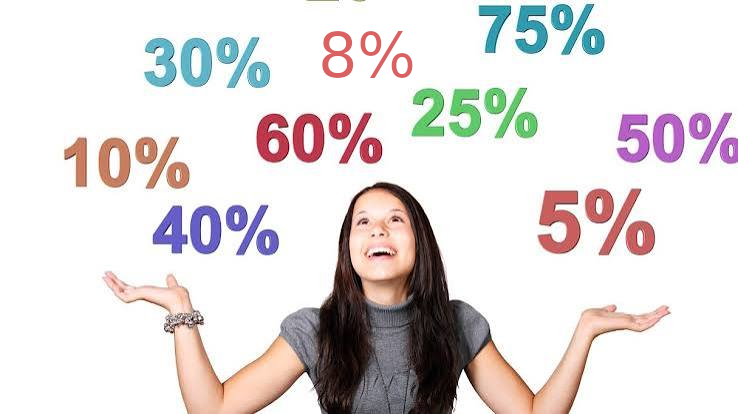
\includegraphics[scale=0.35]{descontos}
		\end{figure}
	\end{frame}
	
	\begin{frame}{Introdução aos conceitos de receita}
		\begin{block}{Custo}
			
		\end{block}
		\begin{block}{Desconto}
			
		\end{block}
	\end{frame}	


\end{document}
